% !TEX TS-program = pdflatex
% !TEX encoding = UTF-8 Unicode

\documentclass[11pt]{article}                                                   % use larger type; default would be 10pt
\usepackage[utf8]{inputenc}                                                     % set input encoding (not needed with XeLaTeX)

%%% PAGE DIMENSIONS ------------------------------------------------------------
\usepackage[top=0.8in, left=1in, right=1in, bottom=0.8in]{geometry}             % to change the page dimensions
\geometry{a4paper}                                                              % or letterpaper (US) or a5paper or....
\usepackage[parfill]{parskip}                                                   % Activate to begin paragraphs with an empty line rather than an indent

%%% HEADERS & FOOTERS ----------------------------------------------------------
\usepackage{fancyhdr}                                                           % This should be set AFTER setting up the page geometry
\pagestyle{fancy}                                                               % options: empty , plain , fancy
\renewcommand{\headrulewidth}{0pt}                                              % customise the layout...
\lhead{}\chead{}\rhead{}
\lfoot{}\cfoot{page \thepage}\rfoot{}

%%% SECTION TITLE APPEARANCE ---------------------------------------------------
\usepackage{sectsty}
\allsectionsfont{\sffamily\mdseries\upshape}                                    % (See the fntguide.pdf for font help)

%%% PACKAGES -------------------------------------------------------------------
\usepackage[font=small,labelfont=bf,textfont=it]{caption}                       % stylize captions
\usepackage{graphicx}                                                           % support the \includegraphics command and options
\usepackage{booktabs}                                                           % for much better looking tables
\usepackage{array}                                                              % for better arrays (eg matrices) in maths
\usepackage{paralist}                                                           % very flexible & customisable lists (eg. enumerate/itemize, etc.)
\usepackage{verbatim}                                                           % adds environment for commenting out blocks of text & for better verbatim
\usepackage{subfig}                                                             % make it possible to include more than one captioned figure/table in a single float
\usepackage{mathtools}                                                          % for math environments like align
\usepackage{amssymb}                                                            % for symbols like \therefore
\usepackage{verbatim}                                                           % for including text as appears, verbatim
\usepackage{listings}                                                           % for including external files as text, eg code
\usepackage{color}                                                              % for coloring of files and images
\usepackage{overpic}                                                            % for adding annotations to pictures
\usepackage[version=3]{mhchem}

%%% EQUATIONS ------------------------------------------------------------------
\numberwithin{equation}{section}                                                % Number equations by section (change for different levels)

%% BIBIOGRAPHY ------------------------------------------------------------------
\usepackage{cite}
\bibliographystyle{unsrt}

%%% ToC (table of contents) APPEARANCE -----------------------------------------
%\usepackage[nottoc,notlof,notlot]{tocbibind}                                   % Put the bibliography in the ToC
%\usepackage[titles,subfigure]{tocloft}                                         % Alter the style of the Table of Contents
%\renewcommand{\cftsecfont}{\rmfamily\mdseries\upshape}
%\renewcommand{\cftsecpagefont}{\rmfamily\mdseries\upshape}                     % No bold!

%%% PDF LINKS AND STYLE --------------------------------------------------------
\usepackage[unicode=true,
    bookmarks=true,bookmarksnumbered=true,bookmarksopen=true,
    bookmarksopenlevel=2, breaklinks=false,pdfborder={0 0 0},backref=false,
    colorlinks=false] {hyperref}                                                % for links in pdf file, no colors
\hypersetup{pdftitle={DOCUMENT NAME},
    pdfauthor={Josh Wainwright}}                                                % set name of document and author here

%%% END Article customizations

%%% Include TIKZ images directly into document ---------------------------------
\usepackage[svgnames]{xcolor}
\usepackage{tikz}
\usetikzlibrary{decorations.markings}
\usetikzlibrary{shapes.geometric}

\newif\iffinal                                                                  % introduce a switch for draft vs. final document
\finaltrue                                                                      % use this to compile the final document
\usepackage{tikz}

\iffinal
    \newcommand{\inputTikZ}[1]{%
        \input{#1}%
    }
\else
    \newcommand{\inputTikZ}[1]{%
        \beginpgfgraphicnamed{#1-external}%
        \input{#1}%
        \endpgfgraphicnamed%
    }
\fi

%%% Include svg images directly in document (requires Inkscape) ----------------
\newcommand{\executeiffilenewer}[3]{%
    \ifnum\pdfstrcmp{\pdffilemoddate{#1}}%
        {\pdffilemoddate{#2}}>0%
        {\immediate\write18{#3}}
    \fi
}
\newcommand{\includesvg}[1]{%
    \executeiffilenewer{#1.svg}{#1.pdf}%
    {inkscape -z -D --file=#1.svg --export-pdf=#1.pdf --export-latex}%
    \input{#1.pdf_tex}%
}

%%% NEW COMMANDS ---------------------------------------------------------------
\renewcommand{\d}{\,\mathrm{d}}                                                 % for integrals
\newcommand{\dx}[2]{\frac{\textrm{d} #1}{\textrm{d} #2}}                        % for derivatives
\newcommand{\dd}[2]{\frac{\textrm{d}^2 #1}{\textrm{d} #2^2}}                    % for double derivatives
\newcommand{\pd}[2]{\frac{\partial #1}{\partial #2}}                            % for partial derivatives
\newcommand{\pdd}[2]{\frac{\partial^2 #1}{\partial #2^2}}                       % for double partial derivatives
\newcommand{\e}[1]{\text{e}^{#1}}                                               % for exponentials
\newcommand{\code}[1]{\texttt{#1}}                                              % for verbatim code view
\newcommand{\inter}[1]{\shortintertext{#1}}                                     % shorter version of intertext
\newcommand{\under}[1]{\underline{#1}}                                          % for vectors etc.

\let\vaccent=\v                                                                 % rename builtin command \v{} to \vaccent{}
\newcommand{\uv}[1]{\ensuremath{\hat{#1}}}                                      % for unit vector
\newcommand{\abs}[1]{\left| #1 \right|}                                         % for absolute value
\newcommand{\avg}[1]{\left< #1 \right>}                                         % for average
\let\underdot=\d                                                                % rename builtin command \d{} to \underdot{}
\newcommand{\ket}[1]{\left| #1 \right>}                                         % for Dirac bras
\newcommand{\bra}[1]{\left< #1 \right|}                                         % for Dirac kets
\newcommand{\braket}[2]{\left< #1 \vphantom{#2} \right|
    \left. #2 \vphantom{#1} \right>}                                            % for Dirac brackets
\newcommand{\matrixel}[3]{\left< #1 \vphantom{#2#3} \right|
    #2 \left| #3 \vphantom{#1#2} \right>}                                       % for Dirac matrix elements
\newcommand{\grad}[1]{\nabla #1}                                                % for gradient
\let\divsymb=\div                                                               % rename builtin command \div to \divsymb
\renewcommand{\div}[1]{\nabla \cdot #1}                                         % for divergence
\newcommand{\curl}[1]{\nabla \times #1}                                         % for curl
\let\baraccent=\=                                                               % rename builtin command \= to \baraccent
\renewcommand{\=}[1]{\stackrel{#1}{=}}                                          % for putting numbers above =


%*******************************************************************************
%******************************** END HEADER ***********************************
%*******************************************************************************

\begin{document}
%!TEX root = mainfile.tex
\begin{titlepage}
  \begin{center}
    \vspace*{\fill}

    \centering
    
\includegraphics[scale=1.0]{Logo.pdf}
    \vfill

    \hrule
    {\LARGE\bf Extragalactic Astrophysics and Cosmology\\Cosmic Reionization \\[0.4cm]}
    \hrule

    \vfill
    \large
    School of Physics and Astronomy\\
    University of Birmingham

    \vfill
    { Joe Baumber,
    	James Bryant,
    	Lewis Clegg,
    	Bethany Johnson,
    	Andrew King,
    	Owen McConnell,
    	Catherine McDonald,
    	Michael O'Neill,
    	Jonathan Shepley,
    	Dorothy Stonell,
    	Rahim Topadar,
    	Josh Wainwright\\}
    \vfill

    \vfill
    \textit{Supervisors:} Graham Smith, Alistair Sanderson, Melissa Gillone \\
    		\vfill
    \textit{Date:} March 2013
    \vfill
    \vfill

    \begin{abstract}
        This study deduces that reionization began at a redshift of $z=17.82$ and ended at a redshift of $z=7\pm 1.8$. This is calculated by directly applying the dynamics of star formation and the ionization rate of neutral hydrogen in the Intergalactic Medium. A photometry strategy consisting of 3 multi-band surveys is proposed in order to observe Lyman Break Galaxies across redshifts 6--17. The surveys will locate $100.5\pm37.0$, $138.7\pm 100.6$, $358.1\pm 158.6$ galaxies in redshift ranges 6--8.5, 8.5--10 and 10--17 respectively. These surveys will be completed by the James Webb Space Telescope and Euclid which are planned for launch in the coming decade. A follow up spectroscopy survey will be used to confirm the redshift and properties of 24, 4 and 48 galaxies in these 3 surveys respectively. The spectroscopy will be carried out using James Webb Space Telescope and a combination of single and multi-slit spectroscopy. It is shown that the use of known gravitational lenses, located between redshift 0.5--0.7, is very beneficial for discovering high redshift candidates as it can increase the depth of surveys by up to 3 magnitudes.
    \end{abstract}


  \end{center}
\end{titlepage}

%\thispagestyle{empty}
%\vspace*{\fill}
%\noindent
%\begin{tabular}{ll}
%\end{tabular}

%\cleardoublepage
%\cleardoublepage

\newpage
\tableofcontents
\newpage
%!TEX root = main.tex

\section{Introduction} % (fold)
\label{sec:introduction}
This experiment involves examining the interactions of neutrons with matter through two experiments using two different detectors. The first detector, a sodium iodide scintillation detector will be used to measure the binding energy of the neutron, and secondly, using a boron-trifluoride counter, measure the moderating properties of water on fast neutrons as a function of radius from a central source.
% section introduction (end)

%!TEX root = main.tex

\section{Experimentation} % (fold)
\label{sec:experimentation}

\subsection{subsection name} % (fold)
\label{sub:subsection_name}
The first experiment that was attempted was measuring the binding energy of neutrons observing the $\gamma$-ray emitted when the neutrons are captured by protons in the water surrounding a neutron source via reaction \ref{eq:neutronbinding},
\begin{align}
	\cf{^{1}_{1}p} + \cf{^{0}_{1}n} &\rightarrow \cf{^{1}_{2}d} + \gamma \label{eq:neutronbinding}
\end{align}

The exact energy would be found from the peak from this photon observed in the spectrum
% subsection subsection_name (end)

\subsection{Calibration} % (fold)
\label{sub:calibration}
Before any data can be read from the spectra taken from the detector, the data has to be calibrated. To do this, a set of known samples with well defined peaks is used to get a relation between the channel number of an observed peak and its energy. Once this is done, a relation can be found that relates the channel number to energy for use on later measurements.

The elements that were used included cobalt, barium, caesium, europium and americium. Each of these elements were available to measure, and each has recorded and accepted peaks that are at well defined positions. The data was taken from the National Nuclear Data Centre (NNDC). The table below shows the data that we collected from these sources. The channel number refers to the position in the spectrum that the peak was observed and the expected peak is the energy of the peak that the respective peak is estimated to correspond to.

\begin{table}[ht]
	\centering
	\begin{tabular}{r c|c|c}
		\multicolumn{2}{c|}{Element} & Channel Number & Expected Peak Energy (keV) \\
		\hline\hline
		Cobolt 		& $\ce{^{60}Co}$  & 369.4	& 1332.0 \\
					&				  & 324.9	& 1173.0	\\
		\hline
		Barium		& $\ce{^{133}Ba}$ & 102.9	& 356.0	\\
					&				  & 86.08	& 302.9		\\
		\hline
		Caesium		& $\ce{^{137}Cs}$ & 188.4	& 661.7 \\
		\hline
		Europium	& $\ce{^{152}Eu}$ & 99.84	& 344.3 \\
					&				  & 222.0	& 778.9		\\
					&				  & 274.9	& 964.1		\\
					&				  & 311.0	& 1121/1086	\\
					&				  & 394.1	& 1408.0	
	\end{tabular}
	\caption{This table shows some data\label{tab:myfirsttable}}
\end{table}

\begin{figure}[ht]
	\centering
	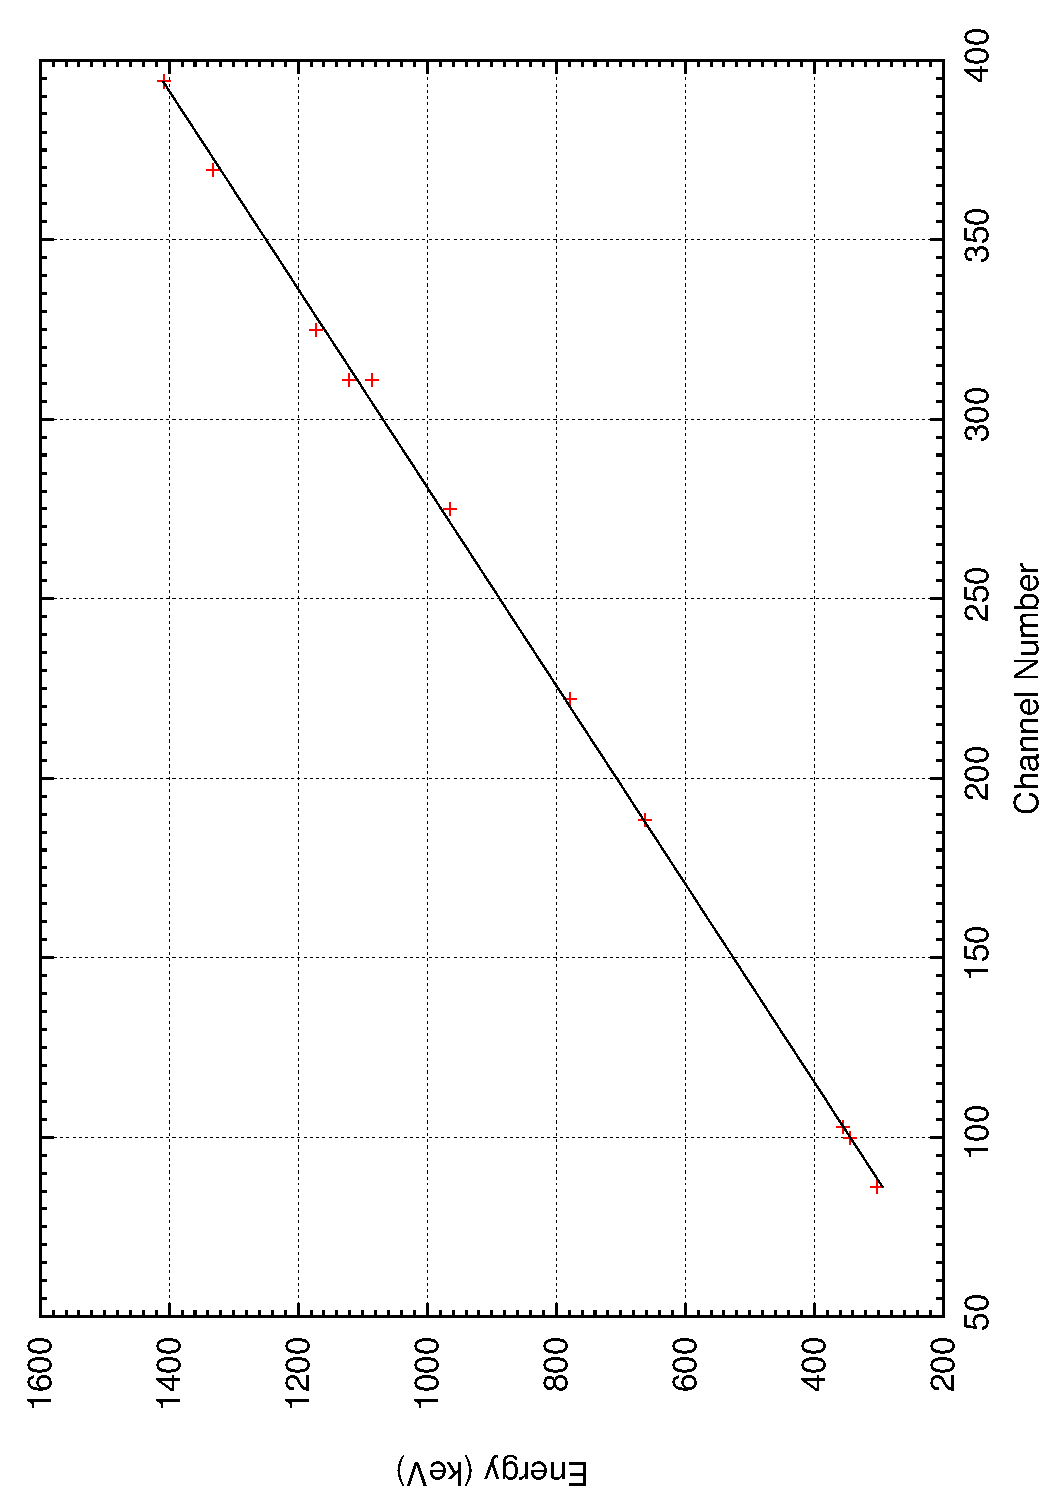
\includegraphics[angle=270,width=0.8\textwidth]{calibration1NaI.pdf}
	\caption{The $\text{BF}_4$ detector uses a high charge to create a flow of ions to measure the incoming neutron. It cannot measure the energy, but simply gives a count for the number of neutrons incident in the detector.\label{fig:bf3detector}}
\end{figure}

% subsection calibration (end)
% section experimentation (end)


\end{document}
    
